\documentclass[../sotsu.tex]{subfiles}

\begin{document}


\section{ルベーグ積分}
\label{sec:lebesgue-integral}


\subsection{可測関数}
\label{sec:measurable-function}

たとえば,以下のような関数だったらどうだろうか.

\begin{definition}
    \label{dfn:simple-function}
    $(X, 𝚺, \mu)$を可測空間とする.
    $E \in 𝚺$をとり,
    さらに$E = E_1 \sqcup \dots \sqcup E_n$と有限個の可測な\refdfn[直和]{dfn:disjoint-union}に分解できるとする.
    $E$上の点で定義された関数$f$が\word{単関数}(simple function)であるとは,
    \begin{equation}
        \label{eq:simple-function}
        f(𝒙) = \sum_{i=1}^{n} \alpha_i \chi_{E_i} (𝒙)
    \end{equation}
    とかけることをいう.
    ここで,$\chi_A (𝒙)$は集合の指示関数,すなわち
    \begin{equation*}
        \chi_A (𝒙) = 
        \begin{cases}
            1  &  𝒙    \in A  \\
            0  &  𝒙 \notin A
        \end{cases}
    \end{equation*}
    である.
\end{definition}

$f$は$E_1$上で$\alpha_1$,$E_2$上で$\alpha_2$の値をとるという単純な関数である.

単関数$f$の積分は,以下のように考えることができる.
話を分かりやすくするために,$E \subset \symbb{R}^2$,$f(𝒙) \geq 0$としよう.
まず$E_1$上での体積は,底面積$\mu(E_1)$×高さ$\alpha_1$である.
$E_2$における体積は,やはり底面積$\mu(E_2)$×高さ$\alpha_2$である.
結果,$E$全体での体積は,
\begin{equation}
    \label{eq:simple-function-volume}
    \sum_{i=1}^{n} \alpha_i \mu(E_i)
\end{equation}
とかけるはずである.


可測関数を定義するために,まず次の記法を導入する.
$E$上で定義された関数$f$に対し,
\begin{equation}
    E\measet{ f > a } \coloneq \Set{  𝒙 \in E  \given  f(𝒙) > a  }
\end{equation}
と定義する.
$E\measet{f<a}$,$E\measet{f\leq a}$なども同様に定義する.

\begin{subequations}

\begin{definition}
    \label{dfn:measurable-function}
    $X$を可測空間,$𝚺$を$\sigma$-加法族とする.
    $f$が\word{$𝚺$-可測},あるいは単に\word{可測}(measurable)であるとは,
    任意の実数$a$に対して,
    \begin{equation}
        \label{eq:measurable-function-gt}
        E\measet{ f > a } \in 𝚺
    \end{equation}
    であることをいう.
\end{definition}

\cref{dfn:measurable-function}と\refdfn-[$\sigma$-加法族]{dfn:sigma-additive-class}の性質から,
まず
\begin{align}
    \label{eq:measurable-function-le}
    E\measet{ f \leq a }  &=  E \setminus E\measet{ f > a }  \in  𝚺  \\
    \label{eq:measurable-function-ge}
    E\measet{ f \geq a }  &=  \bigcap_{n=1}^{\infty} E\measet[\Big]{ f > a - \frac{1}{n} }  \in  𝚺
\end{align}
がいえる.
これらを用いると,
\begin{align}
    \label{eq:measurable-function-lt}
    E\measet{ f < a }  &=  E \setminus E\measet{ f \geq a }  \in  𝚺  \\
    \label{eq:measurable-function-eq}
    E\measet{ f = a }  &=  E\measet{ f \leq a } \cap E\measet{ f \geq a }  \in  𝚺
\end{align}
がいえる.
同様にして,
\begin{align}
    E\measet{ f > -\infty }  &=  \bigcup_{n=1}^{\infty} E\measet{ f > -n }  \in  𝚺  \\
    E\measet{ f < +\infty }  &=  \bigcup_{n=1}^{\infty} E\measet{ f < +n }  \in  𝚺
\end{align}
であり,ここから
\begin{align}
    E\measet{ f = +\infty }  &=  E \setminus E\measet{ f < +\infty }  \in  𝚺  \\
    E\measet{ f = -\infty }  &=  E \setminus E\measet{ f > -\infty }  \in  𝚺
\end{align}
もいえる.

なお,
\cref{eq:measurable-function-gt,eq:measurable-function-ge,eq:measurable-function-lt,eq:measurable-function-le}のうち,
どれを可測関数の定義としても,
残りの3つはそこから導き出せる.

また,
関数$f$が$𝚺$-可測であることを示すとき,
任意の実数$a$に対して$E\measet{f > a}$を示さなくても,
任意の\emph{有理数}$p$に対して$E\measet{f > p}$であることを示せば十分である.
実際,
$a$に収束する単調増加の有理数列$\sequ{p_n}$をとれば\footnote{
    有理数は$\symbb{R}$において\refdfn[稠密]{dfn:dense}であるから,
    このような数列をとることができる.
},
\begin{equation*}
    E\measet{ f > a } = \bigcup_{n=1}^{\infty} E\measet{ f > p_n }
\end{equation*}
とかける.

\cref{eq:simple-function}のような単関数においては,
$E_i = E\measet{ f = \alpha_i }$とかける.
\cref{eq:measurable-function-eq}を使えば,
すべての$i$に対し$E_i \in 𝚺$であるとき,
またその時に限り,\cref{eq:simple-function}は可測である.


\end{subequations}


単関数の積分は,
\cref{eq:simple-function-volume}によって定義できそうである.
一般の可測関数に対する積分も,単関数の形に帰着させることで定義することができる.
そのための準備として,以下を示す.

\begin{theorem}
    \label{thm:measurable-function-to-simple-function}
    測度空間を$(X, 𝚺, \mu)$とする.
    $E \subset X$上で$𝚺$-可測な関数$f$が非負ならば,
    $E$上で$𝚺$-可測であり$f$に各点収束する単調増加の単関数列$\sequ{f_n}$が存在する\cite[定理10.1]{ito-lebesgue-1963}.
\end{theorem}

\begin{figure}[tbp]
    \centering
    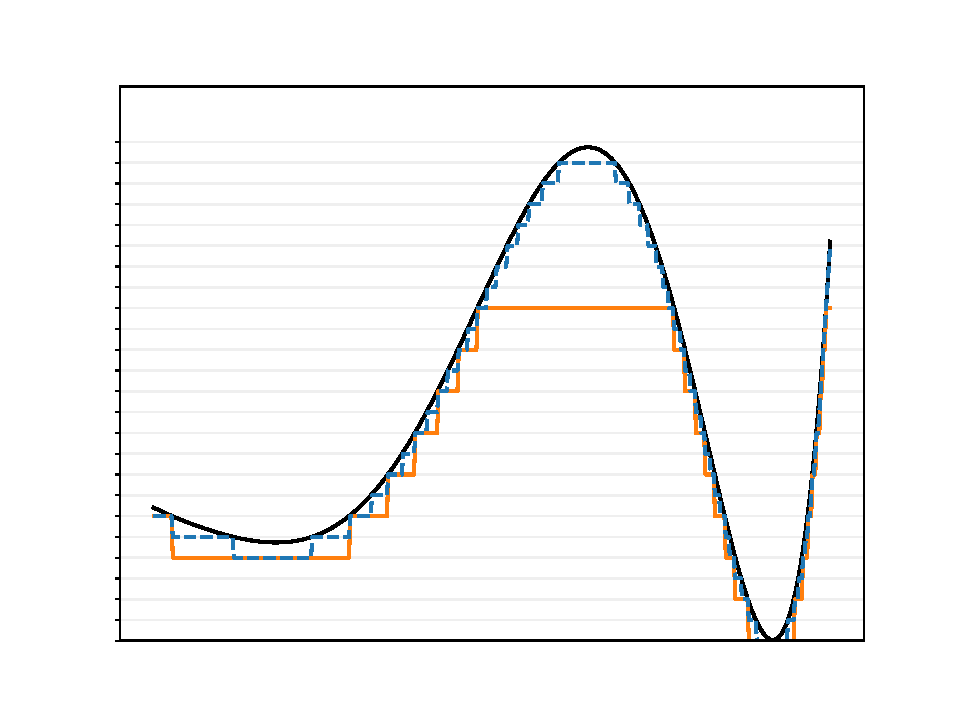
\includegraphics[width=0.7\linewidth]{simple_function.pdf}
    \caption{
        \cref{thm:measurable-function-to-simple-function}における単調増加の単関数列の構成方法.
        赤色の実線が$f_2$である.
        まず$0 \leq f(x) \leq 2$の領域を$2^2 \times 2$等分する横線を引き,
        最も近い横線へと$f(x)$を切り下げる.
        $f_3$(青色の破線)の場合,最初に$0 \leq f(x) \leq 3$の領域を$2^3 \times 3$等分する.
    }
    \label{fig:simple-function}
\end{figure}

\begin{proof}
    \begin{equation*}
        f_n (𝒙) \coloneq 
        \begin{dcases}
            \frac{k-1}{2^n}  &  \text{when} \  \frac{k-1}{2^n} \leq f(𝒙) < \frac{k}{2^n}, \quad \text{where} \  k = 1, 2, 3, \dots, 2^n n  \\
            n  &  \text{when} \  n \leq f(𝒙)
        \end{dcases}
    \end{equation*}
    と定義すれば,これが求めるべき単関数列である(\cref{fig:simple-function}).
    構成よりこれが単調増加であることは明らかである.
    また,$f$が可測であるから,$f_n$も可測である\footnote{
        $f$が可測だから,
        すべての$k$に対し$E_k = E\measet{ f = (k-1)/2^n } \in 𝚺$(\cref{eq:measurable-function-eq})である.
    }.
    最後に$f_n$が$f$に各点収束することを示す.
    まず$f(𝒙) = \infty$となる点$𝒙$については,任意の自然数$n$に対して$f_n (𝒙) = n$であるから,
    $\lim_{n \to \infty} f_n (𝒙) = \infty$.
    そうでなくて,$f(𝒙) < \infty$であれば,
    十分大きな$n$に対して$f(𝒙) < n$となるので,そのような$n$に対して
    $\abs{f_n (𝒙) - f(𝒙)} \leq 1/2^n \to 0$であることからいえる.
\end{proof}





\subsection{ルベーグ積分の定義}
\label{sec:definition-of-Lebesgue-integral}

\cref{sec:measurable-function}で見た可測関数に関して,
ルベーグ積分は次のように定義できる.

\begin{definition}
    \label{dfn:Lebesgue-integral}
    $(X, 𝚺, \mu)$を可測空間,$E \in 𝚺$を可測集合とする.
    \begin{enumerate}
        \item $E = \bigsqcup_{i=1}^{n} E_i$で定義された単関数$f = \sum_{i=1}^{n} \alpha_i \chi_{E_i}$の積分を,
            \begin{equation}
                \label{eq:Lebesgue-integral-for-simple-function}
                \int_E f(𝒙) \ldd{𝒙}
                    \coloneq \sum_{i=1}^{n} \alpha_i \mu(E_i)
            \end{equation}
            で定義する.
        \item $E$で定義された非負関数$f$の積分は,
            $f$に収束するような単関数の単調増加列$\sequ{f_n}$\footnote{
                このような単関数列は,
                たとえば\cref{thm:measurable-function-to-simple-function}によって構成できる.
            }の積分(\cref{eq:Lebesgue-integral-for-simple-function})の極限
            \begin{equation}
                \label{eq:Lebesgue-integral-for-non-negative-function}
                \int_E f(𝒙) \ldd{𝒙}
                    \coloneq \lim_{n \to \infty} \int_E f_n (𝒙) \ldd{𝒙}
            \end{equation}
            と定義する.
        \item $E$で定義された実関数$f$の積分は,
            2つの非負関数
            \begin{align*}
                f^+ (𝒙) = \max \{  f(𝒙), \  0 \},
                \quad
                f^- (𝒙) = \min \{ -f(𝒙), \  0 \}
            \end{align*}
            の\cref{eq:Lebesgue-integral-for-real-function}による積分の差
            \begin{equation}
                \label{eq:Lebesgue-integral-for-real-function}
                \int_E f(𝒙) \ldd{𝒙}
                    \coloneq \int_E f^+ (𝒙) \ldd{𝒙} 
                          -  \int_E f^- (𝒙) \ldd{𝒙}
            \end{equation}
            が定義できるとき\footnote{
                $\int_E f^+ (𝒙) \ldd{𝒙} = \int_E f^- (𝒙) \ldd{𝒙} = \infty$のときを除き,
                \cref{eq:Lebesgue-integral-for-real-function}は定義できる.
            },定積分をもつという.
            さらに\cref{eq:Lebesgue-integral-for-real-function}の値が有限のとき,
            $f$は$E$上で,測度$\mu$について\word{可積分}あるいは\word{積分可能}であるという.
        \item $E$で定義された複素関数$f$の積分は,
            $f(𝒙)$の実部$\Real f(𝒙)$と虚部$\Imaginary f(𝒙)$がともに$E$上で可積分であるとき
            \begin{equation}
                \label{eq:Lebesgue-integral-for-complex-function}
                \int_E f(𝒙) \ldd{𝒙}
                    \coloneq \int_E \Real f(𝒙) \ldd{𝒙} + \iu \int_E \Imaginary f(𝒙) \ldd{𝒙}
            \end{equation}
            と定義する.
    \end{enumerate}
\end{definition}



\subsection{ルベーグ積分の性質}

リーマン積分の場合と同様に,
次のような事柄が成り立つ.

\begin{proposition}
    $f, g$を$E$上で定義された関数とする.
    $A, B \subset E$とし,
    $\alpha, \beta \in \symbb{C}$とする.
    このとき,
    \begin{gather}
        \label{eq:Lebesgue-integral-abs-inequality}
        \int_E \abs{f} \ldd* \leq \abs*{ \int_E f \ldd* }
        \\
        \label{eq:Lebesgue-integral-linearity}
        \int_E (\alpha f + \beta g) \ldd* = \alpha \int_E f \ldd* + \beta \int_E g \ldd*
        \\
        \label{eq:Lebesgue-integral-sqcup}
        \int_{A \sqcup B} f \ldd* = \int_A f \ldd* + \int_B f \ldd*
    \end{gather}
    である.
\end{proposition}

リーマン積分と異なる性質として,
次があげられる.

\begin{proposition}
    $f$を$E$上で可積分な関数とする.
    $g$が$E$上で$f$と\refdfn-[ほとんど至るところ]{dfn:almost-everywhere}一致する関数であれば,
    $g$も$E$上で可積分であり,
    \begin{equation*}
        \int_E f \ldd*  =  \int_E g \ldd*
    \end{equation*}
\end{proposition}

このことは,
$f \neq g$であるような領域$E_0 \subset E$のルベーグ測度がゼロであることから明らかである.


\begin{proposition}[\word{ルベーグの優収束定理}(Lebesgue's dominated convergence theorem)]
    $E$上で$𝚺$-可測な関数の列$\sequ{f_n}$に対して,
    $E$上で可積分である関数$\varphi \geq 0$が存在して$\abs{f_n (𝒙)} \leq \varphi(𝒙)$であり,
    さらに$\sequ{f_n}$が$f$に\refdfn[各点収束]{dfn:pointwise-convergence}するならば,
    \begin{align}
        \lim_{n \to \infty} \int_E f_n (𝒙) \ldd{𝒙} = \int_E f(𝒙) \ldd{𝒙}
    \end{align}
\end{proposition}

\begin{proof}
    \word{ファトゥーの補題}(Fatoe's lemma)を用いて証明する.
\end{proof}



\begin{definition}
    \label{dfn:support}
    ある関数$f \in C(𝛺)$に対し,$f(x) \neq 0$であるような$x \in 𝛺$の集合の\refdfn[閉包]{dfn:closure}
    \begin{equation}
        \supp f  \coloneq  \closureop{ \Set{  x \in 𝛺  \given  f(x) \neq 0  } }
    \end{equation}
    を$u$の\word{台}[だい][だい](support)という.
\end{definition}


\end{document}